%% Introduction %% 

Nous réunissons sous le terme de \enquote{grand public} toutes les populations ne possédant pas d'expertise, de connaissance ou de besoins vis-à-vis des institutions patrimoniales. Ce public couvre donc une population très large et pourtant, dans l'histoire des collections patrimoniales, cette typologie est toujours la dernière à avoir accès à ces collections. 

\subsection{Le dépôt légal, déclencheur de l'accessibilité aux collections patrimoniales}

%% Situer dans le temps %%

C'est le dépôt légal qui par nature, ouvre les collections patrimoniales à toutes les populations. A l'INA, avant sa mise en place, il n'était pas question, pour le grand public, d'avoir accès aux documents que l'institut de l'audiovisuel conservait. A vrai dire, il n'était pas question pour beaucoup de publics d'avoir accès aux images et sons. Comme en témoigne notre documentaliste interrogée. Avant les importants travaux de numérisation dans les années 2000, l'accès aux images et sons conservés par l'INA étaient restreints par leurs supports. En 1993, les documentalistes envoyaient leur commandes par fax aux magasins et ils constataient quelles images avaient été sélectionnées quand elles passaient à la télévision, en même temps que le grand public. Avec le dépôt légal et l'ouverture de l'INAthèque à la BNF François-Mitterand en 1995, le grand public a enfin accès aux diffusions télévisées conservées. 

Malgré tout, le dépôt légal ne signifie pas toujours de l'ouverture au grand public. En 1537, date de la création du dépôt légal des manuscrits, l'ouverture des collections de la bibliothèque royale reste restreinte et il faudra attendre 1720 et l'ouverture de la \enquote{Salle B} à la BNF pour voir une première ouverture à un public \enquote{non-savant}\footnote{Cours d'Initiation aux bibliothèques à l'époque contemporaine de M1 de Technologies numériques appliquées à l'Histoire dispensé par Christine Bénévent}. L'écart des publics au début du dépôt légal de la BNF et de l'INA ne sont certes pas comparables mais ils ont de commun qu'une ouverture au grand public ne signifie pas toujours que le grand public s'aventurera dans les collections de son institution. Les collections patrimoniales s'ouvrent avant tout à un public de chercheurs. En cela les avancées technologiques et leur généralisation dans la société ont contribué à l'ouverture de ces collections et de leur médiation à véritablement tous les publics. Grâce à la numérisation de ces documents et à la démocratisation de l'informatique personnel, les collections numériques des institutions patrimoniales s'invitent à domicile et plus récemment dans nos poches, grâce aux téléphones portables. 

\subsection{Sites web et réseaux sociaux : amener le patrimoine au grand public}

%% Sites web %% 

La principale porte d'entrée aux collections patrimoniales des institutions est la médiation en ligne de leurs collections. Cette ouverture commence par des sites web tels que Gallica\footcite{gallica} en 2000 ou ina.fr\footcite{ina} en 2006. Ces sites proposent une sélection de documents de l'institution, découpés et présentés pour le grand public\footcite[][136]{bermès2024} comme ouvertures aux collections tout en permettant la recherche. 
\begin{figure}[H]
	\centering
	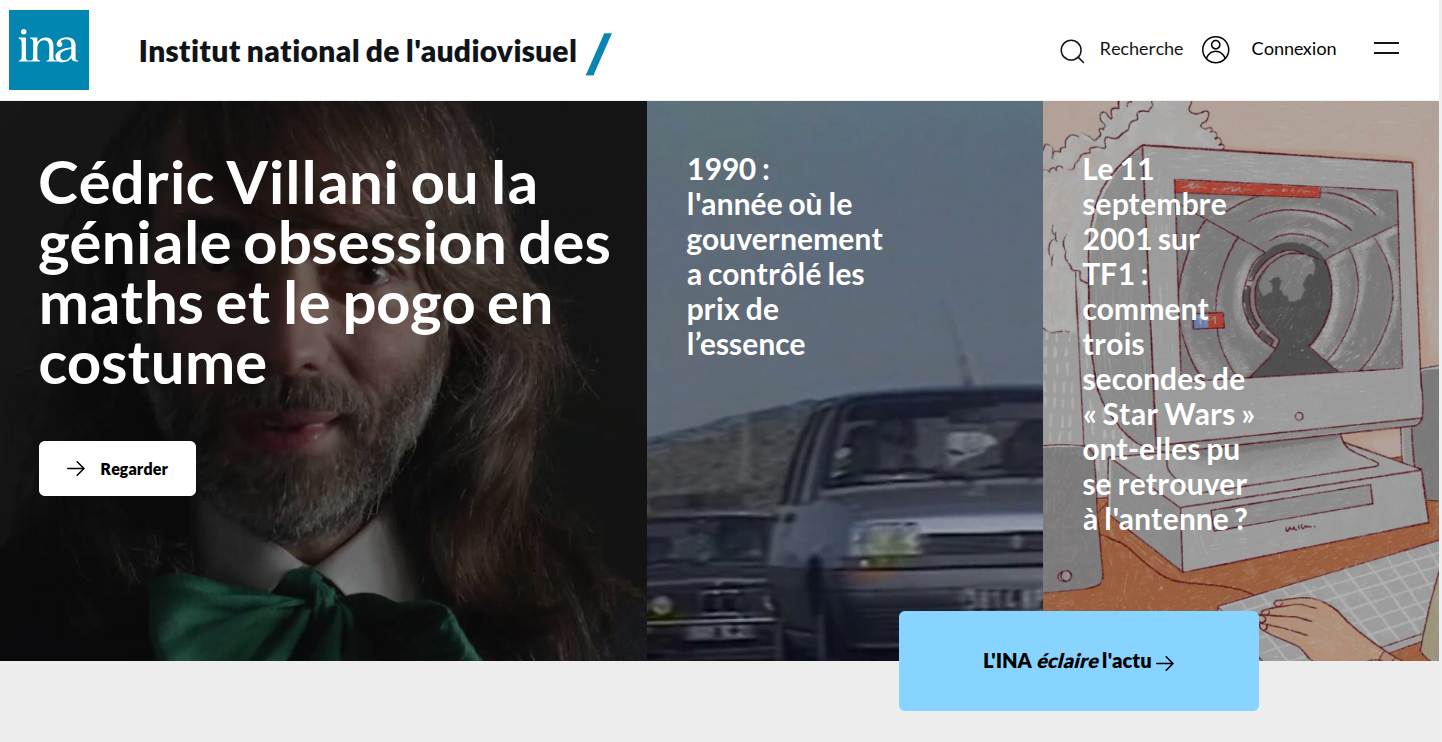
\includegraphics[width=0.75\textwidth]{./illustrations/inafr.png}
	\caption{Capture d'écran de l'accueil du site ina.fr}
	\label{fig:siteweb}
\end{figure}
Pour l'INA, c'est un grand succès, dès son lancement le site trouve son public, qui s'approprie directement les collections. Ils recherchent leurs souvenirs télévisés avec les shadoks, des moments forts de la télévision en cherchant le Général De Gaulle ou plus simplement en recherchant le moment fort de la télévision à la date de leur naissance\footcite[]{zotero-item-158}. 

%% Réseaux sociaux %%

Quelques années plus tard, ce sont avec les réseaux sociaux que ces institutions viennent à la rencontre du grand public. Ils adoptent les codes du web en s'adaptant aux formats courts des réseaux sociaux. En retour, les internautes s'approprient ces documents d'archives. En 2017 la \enquote{carte gastronomique} de la BNF, une carte gastronomique de la France établie par Alain Bourguignon en 1929 connaît un grand succès quand les internautes partagent leur spécialités culinaires locales en ligne sur les réseaux sociaux\footcite[][5]{bertrand2021/mars/15}. Sur les comptes de ces institutions, les équipes d'éditorialisation mettent en scène des évènements d'actualités afin de susciter des réactions chez ce public et à potentiellement susciter de l'intérêt à explorer le reste des collections afin de les rediriger vers des contenus qu'ils ne consulteraient pas spontanément. Récemment, on pouvait voir des utilisateurs des réseaux sociaux s'approprier et parodier les codes des documents de l'INA sur les réseaux\footnote{Les exemples évoqués ont été trouvés sur le réseau social Instagram avec les hashtags \enquote{ina} et \enquote{parodie}}. Dans la continuité des réseaux sociaux il existe un service de l'INA, nommé \enquote{Mediaclip}, un outil clef en main permettant aux créateurs de contenu d'acheter des extraits de documents de l'INA\footcite{zotero-item-708}. Désormais la majorité des institutions patrimoniales ont leur réseaux sociaux afin de toucher un public plus large. Cela comprend les musées comme le Louvre, le musée d'Orsay ou des centres d'archives et ce peu importe la taille de l'institution. Ils fait désormais partie des missions du \gls{td} de permettre de mobiliser ces documents. Par l'intermédiaire des réseaux sociaux, ces documents, quels qu'ils soient, peuvent être mobilisés pour éclairer l'actualité\footcite[][147]{caporiondo-prost2026}, comme l'illustrent ces captures d'écran de publications sur le réseaux social \enquote{Instagram} des archives nationales, de Gallica, du Louvre et de l'INA le 12 août 2026, jour d'éclipse.
\begin{figure}[H]
	\centering
	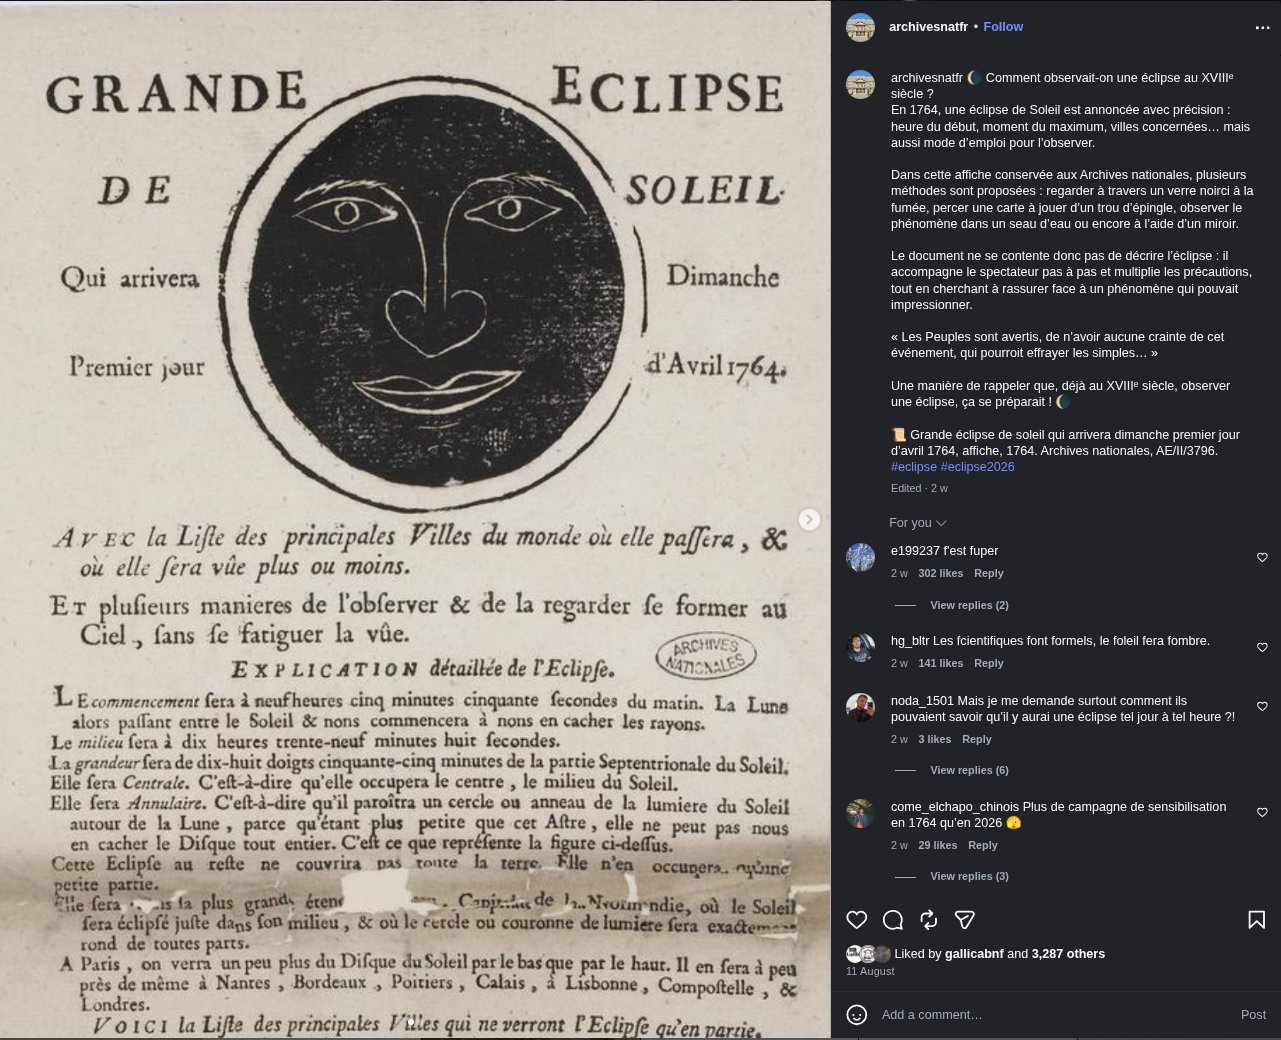
\includegraphics[width=0.24\textwidth]{./illustrations/insta_an.png}\hfill
	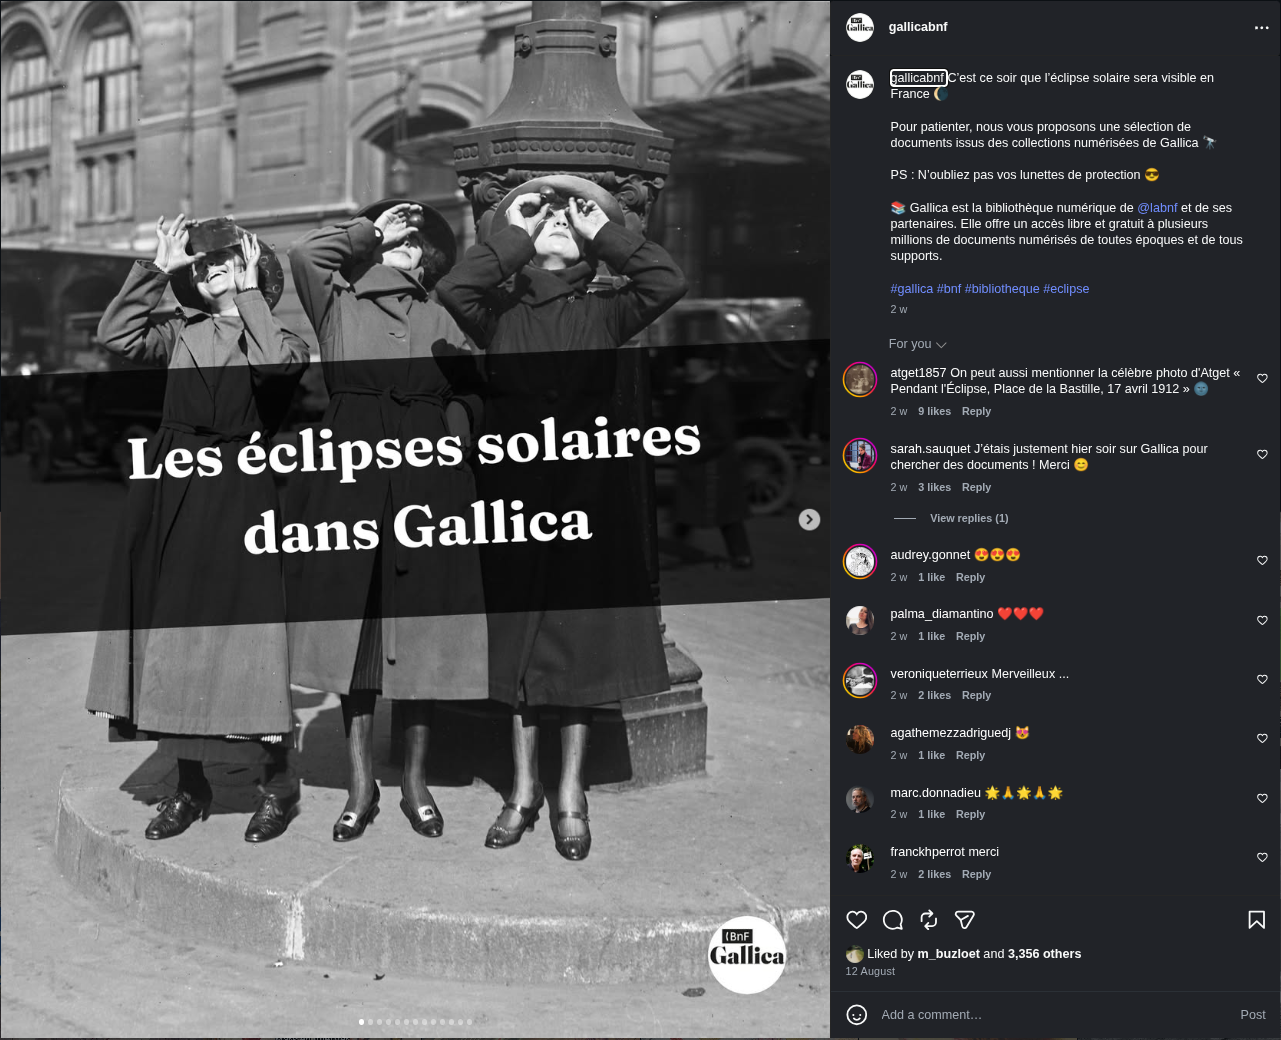
\includegraphics[width=0.24\textwidth]{./illustrations/insta_gallica.png}\hfill
	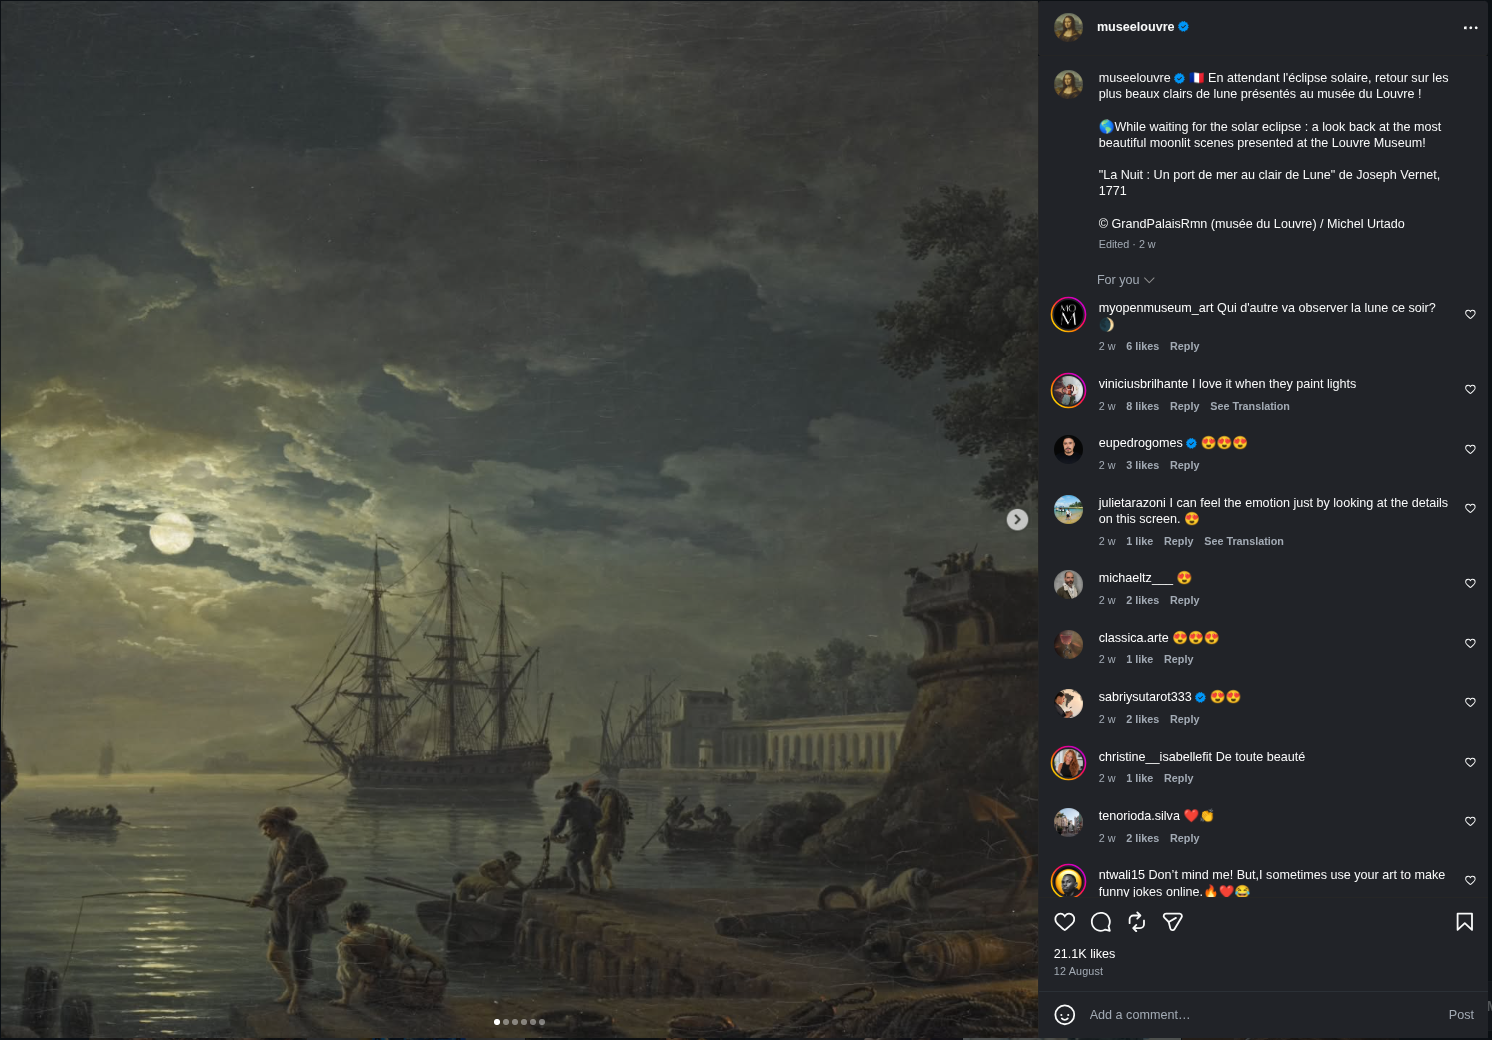
\includegraphics[width=0.24\textwidth]{./illustrations/insta_louvre.png}\hfill
	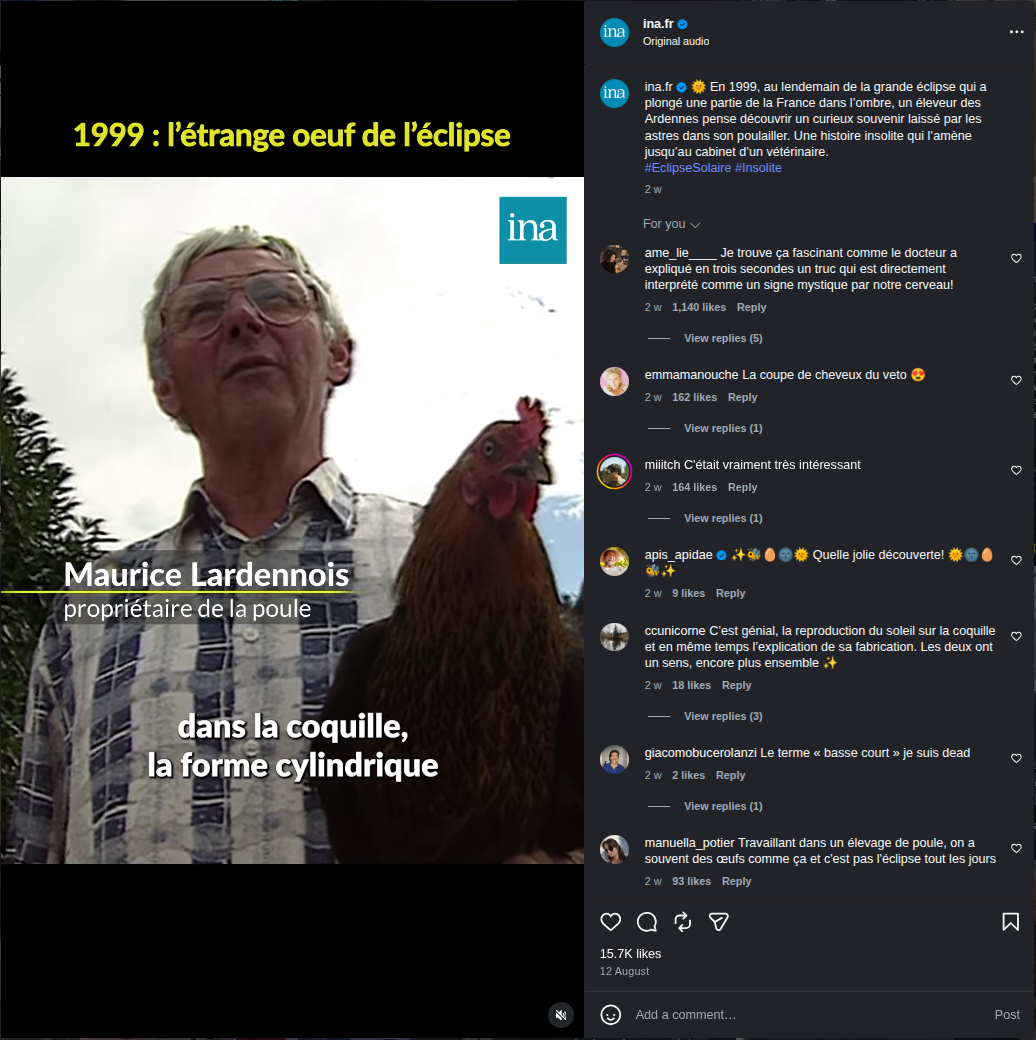
\includegraphics[width=0.24\textwidth]{illustrations/insta_ina.png}
	\caption{Capture d'écran d'une publication du compte officiel des institutions sur instagram le jour de l'éclipse du 12 août 2026 - De gauche à droite : Archives Nationales, Gallica, Louvre, INA}
	\label{fig:insta}
\end{figure}

C'est donc en partie grâce aux réseaux sociaux que le grand public s'est réapproprié ses archives. Au point où aujourd'hui, mêlé à l'innovation de l'intelligence artificielle, ce même grand public, du moins une partie, s'approprie ces documents ou au moins ses codes pour créer de fausses archives. En sa qualité de référent de documents d'archives audiovisuel, l'INA a la responsabilité de sensibiliser les chercheurs au sujet des fausses archives et de l'éthique de la recherche. 

%% Conclusion %%

La conséquence de cette consommation des informations par extraits, via la médiation et l'éditorialisation de l'institution est un public connaissant l'institution, ses collections mais ayant moins de contexte concernant l'archive, sa création, son contexte historique. Cette mode consommation est une véritable rupture, la connaissance ne se transmet plus de la même façon, elle n'est plus recherchée mais découverte. De ce fait, il revient à l'institution et à ses documentalistes de contextualiser et d'apporter le savoir qui accompagne ces documents. Ce public n'est en contact avec les collections que par sa médiation, en conséquent, son accessibilité aux collections ne présente pas d'enjeu important, si ce n'est la responsabilité de l'INA sur la diffusion de fausses archives. Si ce public vient à franchir une salle de lecture, il ne sera plus confronté aux même outils. La confrontation aux bases de données peut être source de frustration en comparaison à la médiation des sites web et réseaux sociaux de l'institution. 